%! TEX root = ../thesis.tex

\chapter{The Pierre Auger Observatory}
\label{chap:auger-observatory}

Located on the argentinian high-plains of Pampa Amarilla, the Pierre Auger observatory is a hybrid detector designed to detect and study cosmic rays of the highest
energies. With an effective area of \SI{3000}{\kilo\meter\squared} it is by far the largest experiment of its kind \cite{DesignReport}.

Altough first proposed in 1992, it took 18 years until the idea of a large scale experiment to detect cosmic rays matured and construction of the first prototype 
started near Mendoza \cite{AugerTimeline}. Some further 20 years later, the Pierre Auger collaboration has co-authored over \TODO publications and continues to 
advance research in astroparticle physics.

It does this via a hybrid approach, combining measurements of a \textbf{S}urface \textbf{D}etector (SD) as well as a \textbf{F}louresence \textbf{D}etector (FD). 
Additional machinery, such as the e\textbf{X}treme (XLF) and \textbf{C}entral \textbf{L}aser \textbf{F}acility (CLF), is installed to monitor atmospheric 
variables. This improves the overall systematic accuracy of predictions made by the experiment. An overview of the site can be seen in \autoref{fig:auger-array}. 
Data measured by the FD, SD and the atmospheric monitors is sent to a \textbf{C}entral \textbf{D}ata \textbf{A}cquisition \textbf{S}ystem (CDAS) located in the 
nearby town of Malargüe.

This chapter offers a brief look into the measurement principle and setup of the observatory. Information regarding the fluoresence detector can be found in 
\autoref{sec:fluoresence-detector}. The SD is described in \autoref{sec:surface-detector}. A more in depth read on detector specifications and design choices is 
represented by the Pierre Auger observatory design report \cite{DesignReport}, where a lot of information stated in this chapter is conglomerated from. Notes on 
the event reconstruction are listed in \autoref{sec:event-reconstruction} and summarized from \cite{SDReconstruction} and \cite{FDReconstruction}.

\begin{figure}
	\centering
	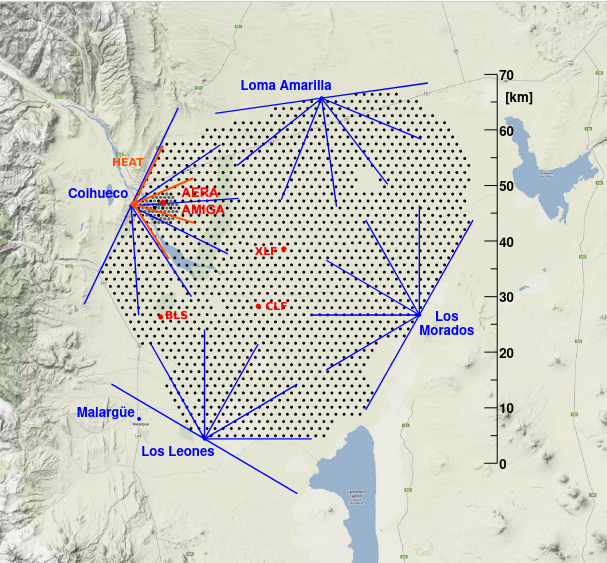
\includegraphics[width=0.9\textwidth]{imgs/auger_array.png}
	\caption{Overview of the Pierre Auger observatory. The four different FD sites (respective FOV shown with blue lines) sit at the edge of the detector area and 
	monitor the night sky above the SD array consisting of 1600 water tanks (black dots). A denser spacing of stations near Coihueco is equipped with additional 
	electronics such as e.g. radio antennas (AERA) and muon detectors (AMIGA). Image taken from \cite{AugerArray}}. \label{fig:auger-array}
\end{figure}

\begin{figure}
	\begin{subfigure}[b]{0.5\textwidth}
		\centering
		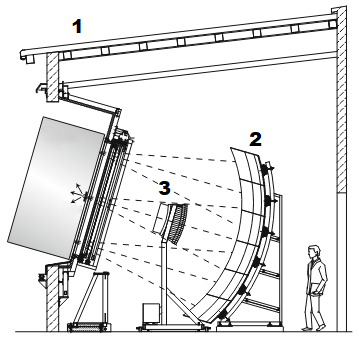
\includegraphics[width=\textwidth]{./imgs/auger_fd.png}
		\caption{\textbf{FD eye setup}}
		\label{fig:fd-eye}
	\end{subfigure}
	\hfill
	\begin{subfigure}[b]{0.5\textwidth}
		\centering
		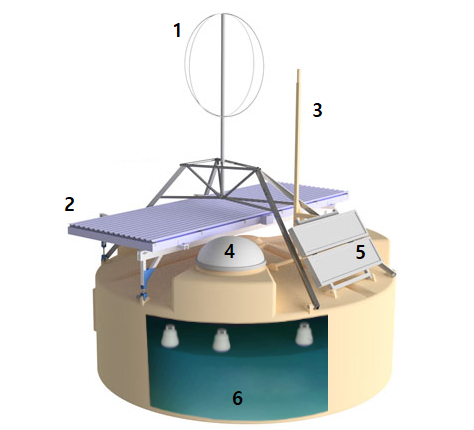
\includegraphics[width=\textwidth]{./imgs/auger_sd.png}
		\caption{\textbf{SD station setup}}
		\label{fig:sd-station}
	\end{subfigure}
	\caption{\textbf{(a)} Schematic view of an FD eye with housing (1), main mirror (2) and camera (3). Image taken from \cite{FDReconstruction} \textbf{(b)} Setup
	of an SD WCD with radio antenna (1), SSD (2), communication and GPS antenna (3), electronics box (4), solar panesl (5) and the WCD (6). Image adopted with 
	changes from \cite{UUBstation} and \cite{waterTank}}
\end{figure}


\section{Fluoresence Detector (FD)}
\label{sec:fluoresence-detector}

The FD consists of a total of 27 fluoresence telescopes (eyes) at 4 different sites. Each eye monitors a \SI{30}{\degree} x \SI{30}{\degree} window of the sky at a
resolution of $\approx \, 0.5 \, \frac{ \text{px} }{ \text{deg}^2 }$. This results in an effective FOV of roughly \SI{180}{\degree} x \SI{30}{\degree} per FD 
station, with an exception of Coihueco, where three additional telescopes - HEAT (\textbf{H}igh \textbf{E}levation \textbf{A}uger \textbf{T}elescope) - are 
installed to enable monitoring of higher zenith angles ($\SI{30}{\degree}\leq\theta\leq\SI{60}{\degree}$) and increase sensitivity for showers of lower energies 
(compare \autoref{chap:physical-background}). A schematic of the setup of each eye is given in \autoref{fig:fd-eye}.

The individual telescopes consist of \SI{3.6}{\meter} by \SI{3.6}{\meter}, convex mirrors. They reflect incoming light onto a set of 440 photomultipliers (PMTs), 
each corresponding to one pixel in the resulting image seen by an eye. Since the setup needs to be extremely sensitive to UV light in order to detect flouresence 
caused by extensive air showers, its operation is limited to the relatively noise free moonless astronomical nights (Sun $\measuredangle$ Horizon 
$\lesssim-18^{\circ}$). When the FD is operational, this allows the observation of the longitudinal propagation of a shower instead of just its' footprint (as seen 
by the SD). 

\section{Surface Detector (SD)}
\label{sec:surface-detector}

The SD consists of 1600 individually operating stations, spaced apart on a hexagonal grid with a standard \SI{1.5}{\kilo\meter} spacing. Each 
station is made up of a main tank filled with \SI{12000}{\litre} of purified water and reflective inner walls, a solar panel and batteries for power management, 
as well as an antenna for communication. Within each tank three PMTs detect Cherenkov light originating from shower particles, these are together with the tank 
referred to as \textbf{W}ater \textbf{C}herenkov \textbf{D}etectors (WCDs). With the (at the time of this work) ongoing AugerPrime upgrade, each station is 
additionally equipped with a \textbf{s}mall \textbf{PMT} (sPMT), \textbf{S}urface \textbf{S}cintillator \textbf{D}etector (SSD), and radio antenna atop the tank.
This allows for the recording of stronger signals, finer separation of electromagnetic and muonic shower component and detection of highly inclined air showers 
respectively \cite{AugerPrime, horandel2019precision}. \autoref{fig:sd-station} shows a schematic blueprint of each SD station.

\subsection{Data acquisition (DAQ)}
\label{ssec:sd-daq}

Onboard electronics, the \textbf{U}pgraded \textbf{U}nified \textbf{B}oard (UUB), or more precisely six 10-bit \textbf{F}lash 
\textbf{A}nalog-to-\textbf{D}igital-\textbf{C}onverters (FADCs) read out measurement data from the PMTs at a sampling rate of \SI{120}{\mega\hertz} 
($\approx\SI{8.33}{\nano\second}$ binning) \cite{verzi2013energy}. This is done in a two-fold way. Three FADCs digitize the PMTs dynode voltage, resulting in the
\textbf{H}igh \textbf{G}ain (HG) output. Three FADCs monitor the anode voltage to form the \textbf{L}ow \textbf{G}ain (LG) output, which can be analyzed if the 
HG output exceeds a value of $2^{10}$ ADC counts and becomes saturated. This effectively enables the measurement of both large ($\geq\mathcal{O}(10^3)$ particles
hitting the tank) as well as small shower signals ($\mathcal{O}(1)$ particle hitting the tank) with sufficient accuracy \cite{SDReconstruction}. Once an FADC bin 
has been recorded and checked for possible triggers (c.f. \autoref{ssec:sd-triggers}) it is written to a ring buffer. If a trigger is issued, the corresponding 
chunk in the ring buffer ($\approx\SI{4.992}{\micro\second}$ (599 bins) before and $\SI{12.07}{\micro\second}$ (1448 bins) after a trigger, $2047 + 1$ bins total),
the measured trace, can be analyzed in order to calibrate a station in the array (\autoref{ssec:online-calibration}, \autoref{ssec:offline-calibration}) or 
processed by a higher-level CPU for event reconstruction purposes (see \autoref{sec:event-reconstruction}).

While each station is equipped with the same electronics and runs the same analysis software, variables like the position in the field, station age or slight 
changes in the manufacturing/installation process cause different stations to age differently. Over the lifetime of the array such differences can sum into 
potentially drastic discrepancies in gathered data. Put simply, an extensive air shower will look different both to different WCDs at the same time as well as 
the same WCD at different times. To account for this, measurements are standardized across all stations. ADC counts are related to a \textbf{V}ertical 
\textbf{E}quivalent of through-going \textbf{M}uons (VEM) that would result in the same signal strength. In this fashion, the maximum response that is generated 
by a PMT from one vertically through-going muon is defined as \SI{1}{\Peak}. The total deposited charge (equivalent to the integral of the response) is defined 
as \SI{1}{\Charge}. The conversion factor between ADC counts and VEM$_\text{Peak}$ and VEM$_\text{Ch.}$ (referred to as \Ipeak and \Qpeak respectively) is 
estimated from data and continuously updated separately for each station. Note that due to the limited computational resources of the WCD, as well as constraints
on the amount of data that can be transmitted per station in the SD array (\SI{1200}{\bit\per\second}, \cite{localStationCalib}), a simplified, rate-based approach 
is implemented for autonomous calibration in the field (Online calibration), this stands in contrast to the more physics-driven histogram method used during event 
reconstruction (Oflline calibration). In any case, both algorithms are listed in the following subsections and discussed in more detail in the referenced 
literature.

\subsection{Offline calibration}
\label{ssec:offline-calibration}

\subsubsection{Baseline estimation}
\label{sssec:offline-baseline-estimation}

In order to estimate \Ipeak and \Qpeak of a WCD tank first the baseline - the average response in the absence of any signals - of each PMT needs to be determined. 
All further analysis will then be based on the baseline-subtracted PMT data.

For event reconstruction, a first baseline estimate of a WCD PMT is predicted by examining the beginning and end of a 2048 bin ($\SI{17.06}{\micro\second}$) long 
trace. The mode $m$ as well as standard deviation $\sigma$ of the first (last) 300 bins is calculated. All bins larger or smaller than $m\pm2\sigma$ are truncated 
and removed from the trace window. The value of $m$, $\sigma$ is consequently updated and the procedure repeated until a convergence is reached and no further cut 
is necessary. The best estimate $B_\text{front}$ ($B_\text{end}$) for the front (end) of the trace at this point is given by the mean value of all remaining bins. 
It's statistic uncertainty $\sigma_{B_\text{front}}$ ($\sigma_{B_\text{end}}$) is given by the standard deviation of the remaining bins \cite{tobiasBaseline}. The 
baseline between the flat front and end estimate is then interpolated based on the difference 

\begin{equation}
	\Delta B = B_\text{end} - B_\text{front}.
\end{equation}

\begin{itemize}
	\item \textbf{Rejection of anomalous upward fluctuations} $\mathbf{\frac{\Delta B}{\sigma_{\Delta B}} \geq +10}$:

	$B_\text{end}$ being higher than $B_\text{front}$ often indicates errors in the electronic readout or defect components in the measurement chain. There 
	exists no physical reason why the end baseline should be (significantly) higher than the front. Consequently, traces where this is the case are ignored 
	during event reconstruction.

	\item \textbf{Constant approximation for small upward fluctuations} $\mathbf{+5 > \frac{\Delta B}{\sigma_{\Delta B}} \geq 0}$:

	Small fluctuations of the baseline are expected and the norm. If these fluctuations are positive ($B_\text{end} > B_\text{front}$) the method of 
	calculating the mode, truncating outliers and repeating both steps is applied to the entire length of the signal, resulting in a constant baseline estimate
	$B$ across the trace.

	\item \textbf{Step-function approximation for small downward fluctuations} $\mathbf{0 > \frac{\Delta B}{\sigma_{\Delta B}} \geq -1}$:

	Unlike positive fluctuations, negative fluctuations ($B_\text{end} < B_\text{front}$) can have a physical significance. Due to the undershoof of PMTs after
	detecting a signal in the WCD (compare \cite{glietta2008recovery}), the baseline estimate decreasing towards the end of the trace often indicates the 
	presence of shower particles within the tank. For this reason, downward fluctuations are handled differently from upward ones. If the fluctuations are 
	sufficiently small, the baseline across the trace is estimated as a simple step-function; The trace is separated into two parts along its' maximum ADC 
	value. The front part (i.e. before the max. value) has the baseline $B_\text{front}$, while the rear part is estimated by $B_\text{end}$. An example of 
	this is shown in \autoref{fig:baseline-step-function-approximation}.

	\item \textbf{Charge-linear approximation for large undershoots} $\mathbf{-1 \geq \frac{\Delta B}{\sigma_{\Delta B}}}$:

	For larger undershoots, the baseline is estimated bin by bin based on the deposited charge in the detector. Starting with a value of $B_\text{front}$ for 
	the bins 1-300, the remaining baseline is first linearly interpolated according to \autoref{eq:baseline-charge-linear-interpolation},

	\begin{equation}
	\label{eq:baseline-charge-linear-interpolation}
		b_i = B_\text{front} - \Delta B \cdot \frac{i - 300}{1448}, \qquad 300 \geq i \geq 2048,
	\end{equation}	

	where the magic numbers 300 and 1448 refer to the last bin of the front baseline estimate and the length of the interpolated baseline respectively. From 
	this, the deposited charge $q_i$ up to bin $i$ can be calculated as per \autoref{eq:deposited-charge}.

	\begin{equation}
	\label{eq:deposited-charge}
		q_i = \sum_{k = 0}^{i} \left( T_k - b_k \right)\exp\left(-\frac{\SI{8.33}{\nano\second}}{\tau}\cdot(i-k)\right)
	\end{equation}
	
	In \autoref{eq:deposited-charge}, $T_k$ refers to the numerical value of bin $k$. Note that an exponential falloff term has to be added to account for the
	decay in signal undershoot with a decay time of $\tau = \SI{45}{\micro\second}$. The value of $\tau$ is determined in \cite{tobiasBaselineUUB}. Assuming 
	the magnitude of the signal undershoot is directly proportional to the deposited charge $q$, a correction of the baseline thus becomes

	\begin{equation}
	\label{eq:baseline-correction}
		b_i = B_\text{front} + \frac{q_i}{q_{1898}} \cdot \Delta B.
	\end{equation}
	
	The parametrization in \autoref{eq:baseline-correction} is chosen such that the charge-interpolated baseline at bin $1898$ (the center position in the last
	$300$ bins) is exactly equal to the rear baseline estimate $B_\text{end}$. The prediction can be made more accurate by repeating the above steps, each time
	recalculating $q_i$ and readjusting the baseline $b_i$ in the process. \autoref{fig:baseline-charge-linear-interpolation} shows an example baseline 
	estimate after three such iterations. In general, it converges to a robust estimate within five repetitions \cite{tobiasBaselineUUB}.

\end{itemize}

\begin{figure}
	\begin{subfigure}[b]{0.5\textwidth}
		\centering
		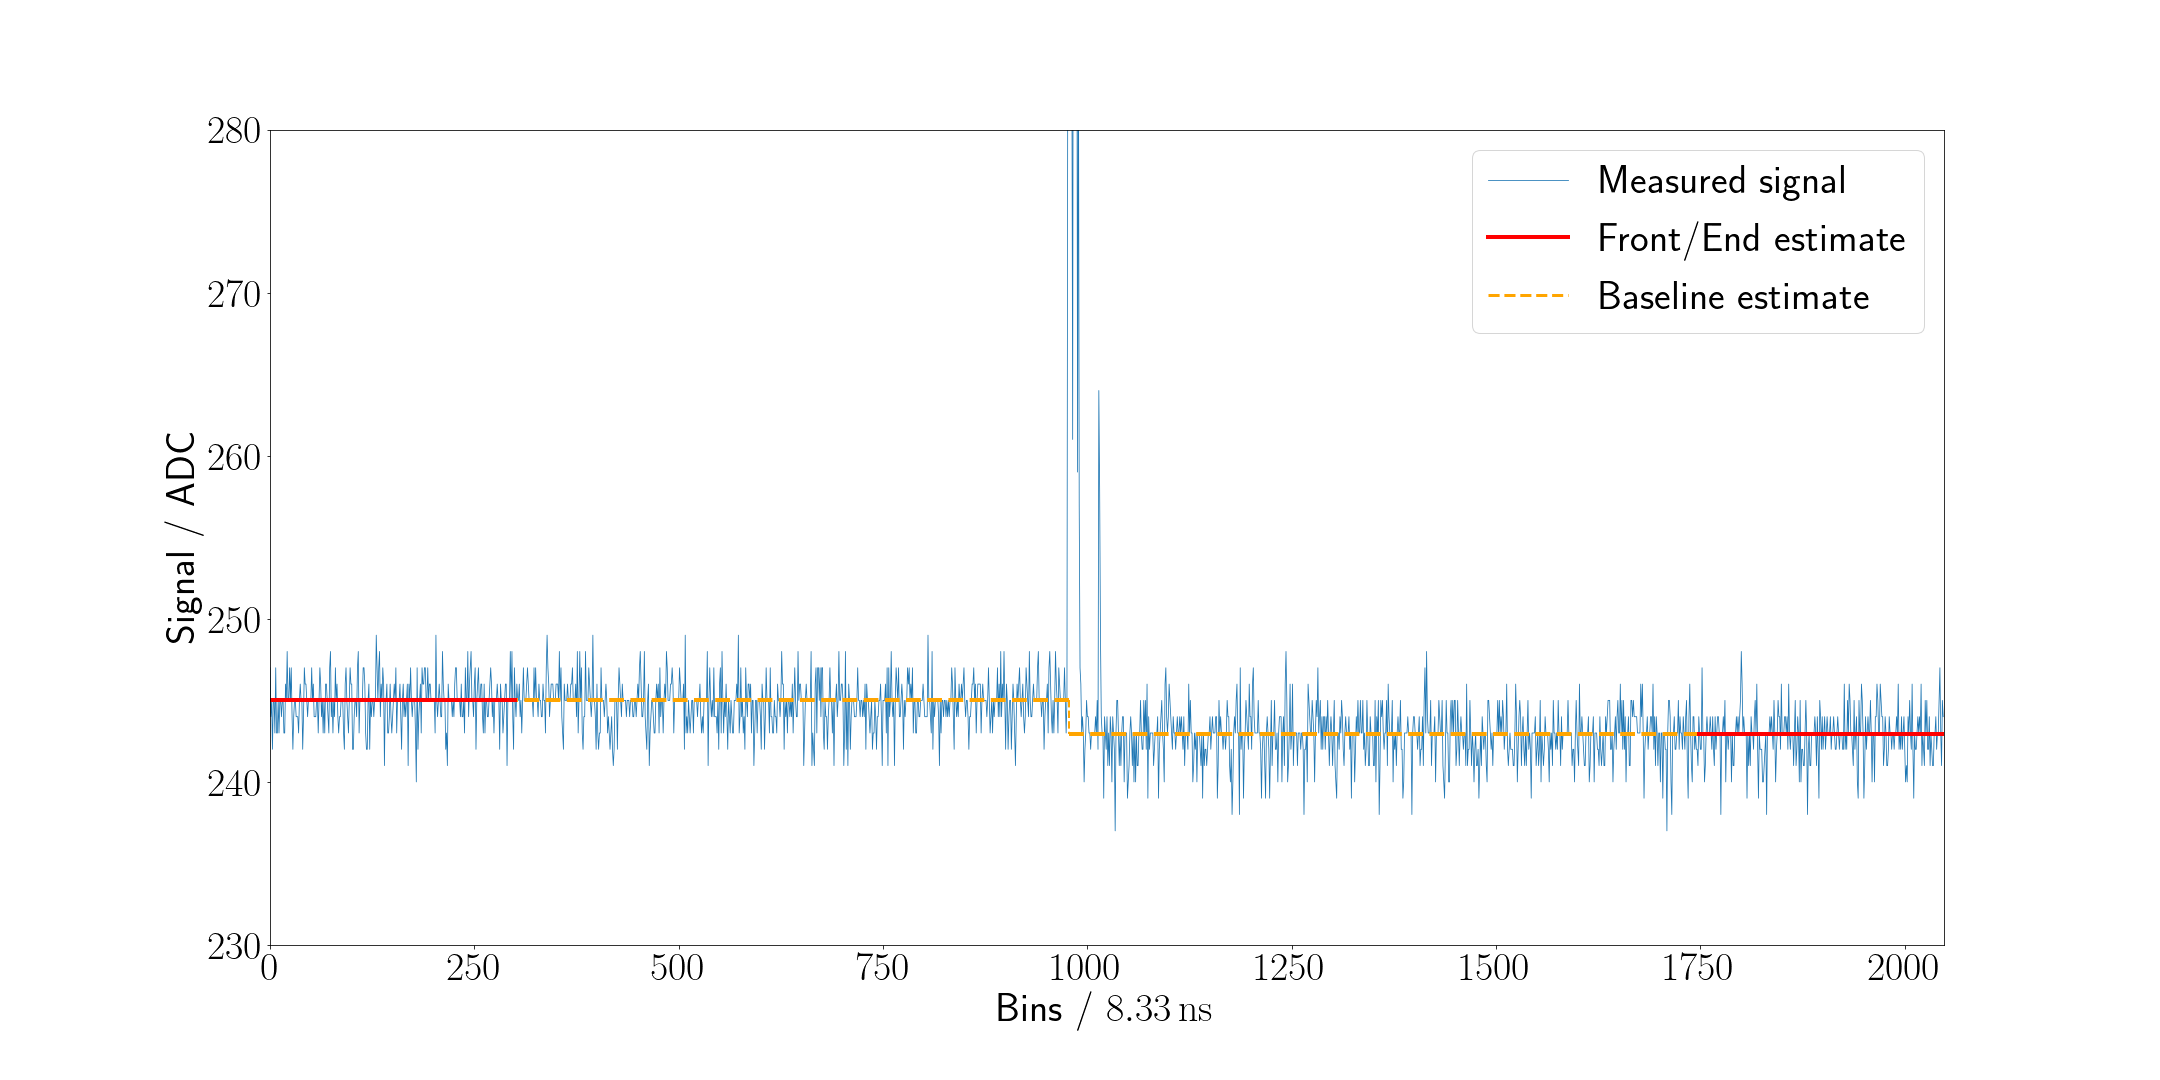
\includegraphics[width=\textwidth]{./plots/baseline_step_function.png}
		\caption{\textbf{Step-function approximation}}
		\label{fig:baseline-step-function-approximation}
	\end{subfigure}
	\hfill
	\begin{subfigure}[b]{0.5\textwidth}
		\centering
		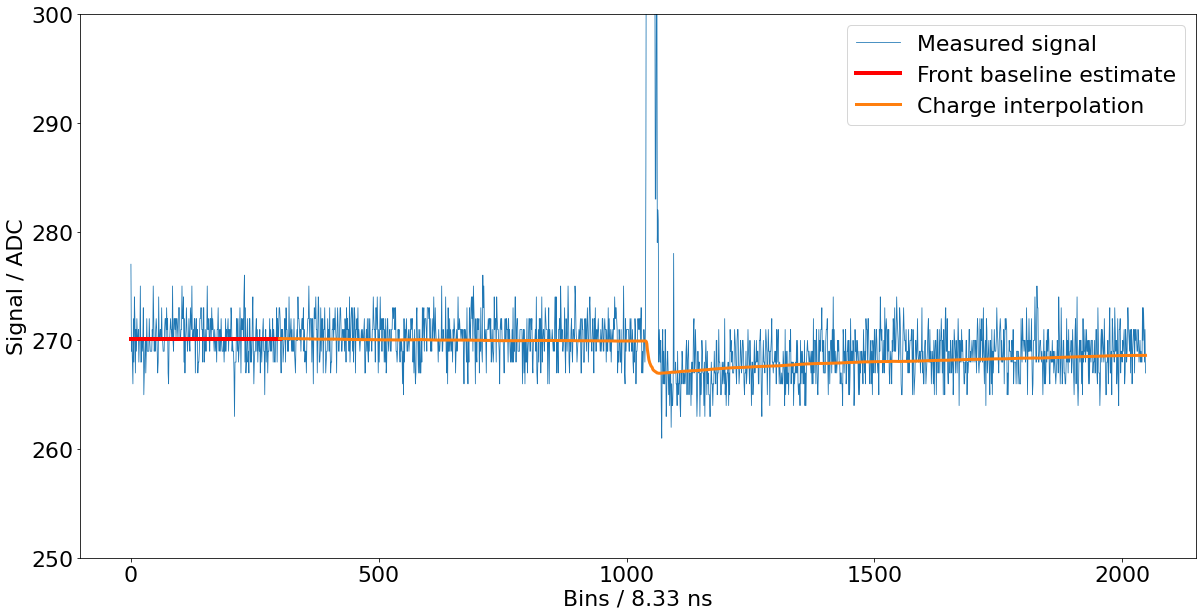
\includegraphics[width=\textwidth]{./plots/baseline_charge_interpolation.png}
		\caption{\textbf{Charge-linear interpolation}}
		\label{fig:baseline-charge-linear-interpolation}
	\end{subfigure}
	\caption{\textbf{(a)} A simple step function is	sufficient to accurately model a PMTs' noise level at small downward fluctuations. \textbf{(b)} For larger 
	discrepancies the more involved charge-linear interpolation is used. Note that the signal undershoot is exaggerated for visualization purposes in both 
	examples.}
\end{figure}

\subsubsection{Estimation of \Ipeak and \Qpeak}
\label{sssec:offline-vem-calibration}

The conversion factor between ADC counts and VEM$_\text{Peak}$, VEM$_\text{Ch.}$ are built from distributions of traces that satisfy the muon trigger, which scans
incoming ADC bins for a value exceeding the muon threshold $t_\upmu = b + \SI{30}{\ADC}$, \SI{30}{\ADC} above baseline, for any of the three WCD PMTs. If this 
requirement is met, 69 bins (19 before, trigger bin, 49 after) are written to the muon buffer, a FIFO (first-in-first-out) type memory storage, that is
subsequently filled with low-energy events, which (in general) didn't satisfy any other trigger but still contain useful information \cite{localStationCalib}.

By histogramming the maximum value (sum) of each trace, the plot shown in \autoref{fig:offline-vem-peak} (\autoref{fig:offline-vem-charge}) can be obtained. It 
becomes apparent that the number of events per bin largely follows a power law with negative spectral index. This is expected considering the discussion in 
\autoref{chap:physical-background}. Noteable are characteristic deviations from this powerlaw, as these contain information about \Ipeak and \Qpeak:

\begin{itemize}
	\item Low energy events from e.g. $e^-$, $e^+$ that deposit their entire energy in the tank give rise to a surplus of events at lower ADC values.
	\item A characteristic (muon) hump appears in the bins $20 - 70$. This surplus is caused by omni-directional muons impinging onto the detector. Since the 
	energy deposited by such muons is roughly constant, the center of the muon hump serves as an estimate of \Ipeak (\Qpeak).
	\item (Not depicted in \autoref{fig:offline-calibration}) In similar plots from related works (c.f. \cite{localStationCalib, streich2018performance}) a
	drastic increase in bin occupations towards the tail end of the histograms can be observed. This is attributed to an increased bin size from \SI{1500}{\ADC} 
	counts onwards, which reduces the amount of data per station sent to CDAS. In the example plots referenced here, a constant binning is chosen instead. 
	This difference is mentioned here to avoid possible confusion. 
\end{itemize}

In this fashion, the average response of the WCD to a through-going muon can be estimated by e.g. fitting a gaussian distribution to the muon hump. However, 
there exists a systematic difference between the response to a vertical or an omni-directional muon. Consequently, correctional factors need to be applied to the 
analysis results. These have been determined in previous experiments \cite{allison2002surface}. Finally, one arrives at an estimate for the conversion factor 
between ADC counts and VEM$_\text{Peak}$, VEM$_\text{Ch.}$.

\begin{figure}
	\begin{subfigure}[b]{0.5\textwidth}
		\centering
		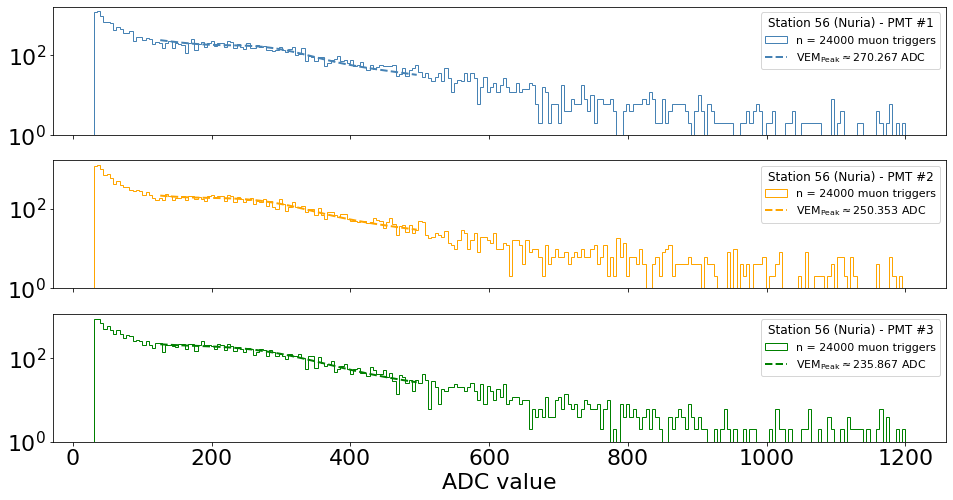
\includegraphics[width=\textwidth]{./plots/offline_vem_peak.png}
		\caption{\textbf{VEM}$_\textbf{Peak}$ \textbf{Histogram}}
		\label{fig:offline-vem-peak}
	\end{subfigure}
	\hfill
	\begin{subfigure}[b]{0.5\textwidth}
		\centering
		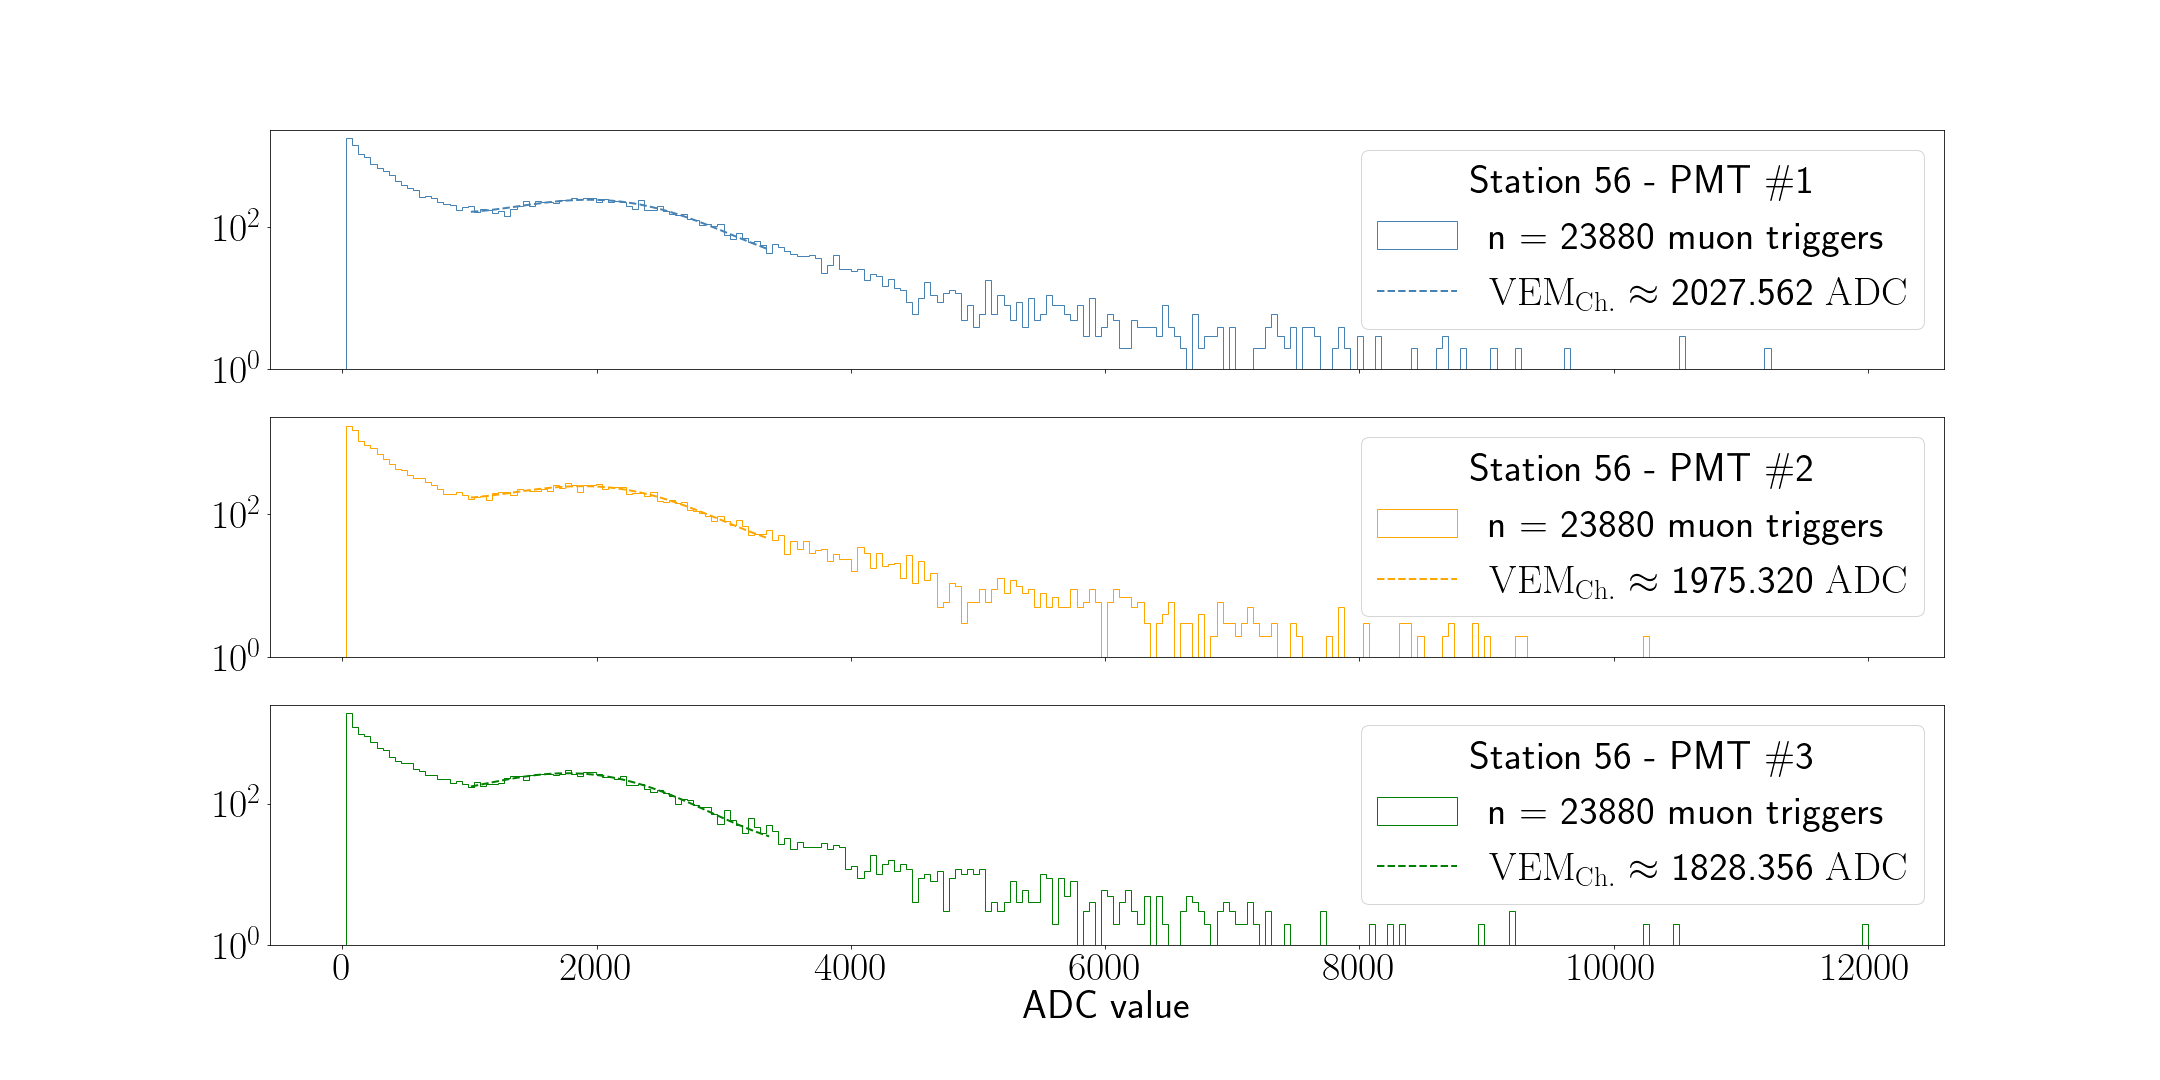
\includegraphics[width=\textwidth]{./plots/offline_vem_charge.png}
		\caption{\textbf{VEM}$_\textbf{Ch.}$ \textbf{Histogram}}
		\label{fig:offline-vem-charge}
	\end{subfigure}
	\caption{\textbf{(a)} The maximum value of each muon trace is histogrammed in order to gain information about the current value of \Ipeak of a station. 
	\textbf{(b)} The conversion factor from recorded ADC values to \Qpeak is given from the histogrammed sum of each muon trace.}
	\label{fig:offline-calibration}
\end{figure}

\subsection{Online calibration}
\label{ssec:online-calibration}

\subsubsection{Baseline estimation}
\label{sssec:online-baseline-estimation}

Each SD station has an autonomous estimate of its' three WCD PMT baselines. They are defined simply as the mean of all first bins for each trace contained in the 
respective muon buffers (see \autoref{sssec:offline-vem-calibration}). This baseline estimate is used to set the thresholds of the hardware triggers discussed in 
\autoref{chap:hardware-triggers}.

\subsubsection{Estimation of \Ipeak and \Qpeak}
\label{sssec:offline-vem-calibration}

Due to the limited computational resources in each station, the determination of \Ipeak and \Qpeak at station-level is fairly naive. Nevertheless, the 
$\sigma$-$\delta$-method shown here has proven to be incredibly robust over the lifetime of the SD array \cite{DesignReport}. 

In the beginning, the to-be-estimated value $I_\text{Peak}^\text{est.}$ ($Q_\text{Peak}^\text{est.}$) is set to the same, predefined value for all PMTs. A simple
single-bin calibration trigger requiring all available WCD PMTs to be above a threshold of $t_{70} = 1.75\,I_\text{Peak}^\text{est.}$ above baseline plus a given 
PMT exceeding $2.5\,I_\text{Peak}^\text{est.}$ is used to determine a calibration trigger rate. If for some reason not all three WCD PMTs are functional, the 
thresholds are altered according to \autoref{tab:calib-trigger-thresholds}. What follows is an iterative procedure to approximate \Ipeak (\Qpeak):

\begin{enumerate}
	\item Calculate the trigger rate $r_\text{cal.}$ of the calibration trigger over a time $t_\text{cal.} = \SI{5}{\second}$.
	\item Adjust $I_\text{Peak}^\text{est.}$ ($Q_\text{Peak}^\text{est.}$) by $\pm\delta$ if $\pm(r_\text{cal.}-\SI{70}{\hertz})\geq\SI{2}{\hertz}$, with
	$\delta = \SI{1}{\ADC}$ initially.
	\item If $t_\text{cal.} < \SI{60}{\second}$ increase $t_\text{cal.}$ by \SI{5}{\second}. If $\delta > \SI{0.1}{\ADC}$ decrease $\delta$ by \SI{0.1}{\ADC}.
	\item While $t_\text{cal.} < \SI{60}{\second}$ jump to step 1, else return $I_\text{Peak}^\text{est.}$ ($Q_\text{Peak}^\text{est.}$).  
\end{enumerate}

\begin{table}[h]
	\begin{center}
	\caption{}
	\begin{tabular*}{0.2\textwidth}{@{\extracolsep{\fill}} cc}
		\toprule
		$n_\text{PMT}$ & $t_{70}$ \\
		\midrule
		1 & 2.85 \\
		2 & 2.00 \\
		3 & 1.75 \\
		\bottomrule
	\label{tab:calib-trigger-thresholds}
	\end{tabular*}
	\end{center}
\end{table}

\section{Event Reconstruction}
\label{sec:event-reconstruction}

If an event has been detected (\autoref{ssec:trigger-procedure}) it is reconstructed at CDAS level, where information from all relevant detectors is conglomerated.
From the reconstructed shower footprint in the SD array as well as the (if available) longitudinal profile measured by the FD stations follows an estimate on 
arrival direction (\autoref{ssec:arrival-direction}), energy (\autoref{ssec:energy-estimation}) and primary particle (\autoref{ssec:primary-particle})

\subsection{Trigger procedure}
\label{ssec:trigger-procedure}

The flux of cosmic rays espically at the highest energies is barely of the order of \SI[per-mode=reciprocal]{1}{\per\kilo\meter\squared\per\year} 
\cite{hillas1984origin}. Consequently, most signals observed by the Auger observatory stem from low-energy cosmic muons and not extensive air showers. This is 
reflected in the hierarchical structure of the triggers, which effectively reject such events. The overall event detection is split up into three tiers, T1, T2 and
T3, where T3 implies the detection of an extensive air shower by either the FD or the SD (or both).

\subsubsection{T1 trigger}
\label{sssec:t1-trigger}

T1 level triggers are implemented at the lowest possible level. This means each FD eye or each SD station raises T1 triggers autonomously. They serve as a first 
indicator on whether or not a signal of any kind is present. For the most part, this is realised by checking for elevated signal strengths, i.e. for hot pixels 
in a FD telescopes image or PMT outputs of an SD station that are significantly above baseline. The respective trigger thresholds are calibrated such that the 
nominal trigger rate during operation is roughly \SI{100}{\hertz} \cite{FDReconstruction, SDReconstruction}. 

\subsubsection{T2 trigger}
\label{sssec:t2-trigger}

T2 level triggers occur at the same location as T1-type triggers. They are different in their more stringent conditions on the signal size or shape. This for 
example entails track shape identification for the FD telescopes, where straight tracks (see \autoref{fig:fd-straight-tracks}) of hot pixels are identified. 
If the resulting pixel track passes an additional quality cut that rejects e.g. lightning signals, the T2 is directly promoted to a T3 trigger ($=\text{Event}$). 
For the SD, an exact discussion of T2 triggers is given in \autoref{sec:hardware-triggers-implementation}. A single tank on average records T2-type events at a 
rate of \SI{20}{\hertz} and forwards this information to the CDAS along with a timestamp. There, incoming information of all tanks is scanned for spatial and 
temporal correlations, which indicate the presence of an extensive air shower. 

\begin{figure}
	\centering
	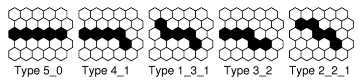
\includegraphics[width=0.8\textwidth]{./imgs/FD_straight_tracks.png}
	\caption{Fundamental shape of tracks that are considered straight. Image from \cite{FDReconstruction}.}
	\label{fig:fd-straight-tracks}
\end{figure}

\subsubsection{T3 trigger}
\label{sssec:t3-trigger}

T3 type triggers, or event type triggers are (with the exception of FD events, which have already been discussed) built from distributions of at least three SD 
stations next to each other that recorded a T2 trigger in close succession. Upon the detection of such a pattern a readout command is issued to nearby stations. If
they observed a T1/T2 

\subsection{Arrival direction}
\label{ssec:arrival-direction}

\subsection{Energy estimation}
\label{ssec:energy-estimation}

\subsection{Primary particle}
\label{ssec:primary-particle}


